\documentclass[a4paper]{scrartcl}

\usepackage[usenames,dvipsnames]{xcolor}
\usepackage{amsmath,amssymb,amsfonts}
\usepackage{graphicx}

\title{Camera Based 2D Feature Tracking ReadMe}
\author{Philipp Rapp}
\date{\today}

\begin{document}

\maketitle

\section*{Mid-Term Report}
\subsection*{MP.0 Mid-Term Report}
\textcolor{gray}{\textit{Provide a Writeup / README that includes all the rubric points and how you addressed each one. You can submit your writeup as markdown or pdf.}}

The document at hand represents the readme file.

\section*{Data Buffer}
\subsection*{MP.1 Data Buffer Optimization}
\textcolor{gray}{\textit{Implement a vector for dataBuffer objects whose size does not exceed a limit (e.g. 2 elements). This can be achieved by pushing in new elements on one end and removing elements on the other end.}}

In order to solve this task, I decided to implement a ring buffer.
A ring buffer can be implemented by creating a plain array with a fixed capacity (in this case 2 elements)
and keeping track of
\begin{itemize}
	\item the current first entry (the head) and
	\item the occupied slots (the size).
\end{itemize}
In order to have reusable code, I used a template for both the data type as well as
for the capacity.
In order to have the same ease of use as for the STL vector, I also implemented a (non-complete)
iterator class for the ring buffer.

\section*{Keypoints}
\subsection*{MP.2 Keypoint Detection}
\textcolor{gray}{\textit{Implement detectors HARRIS, FAST, BRISK, ORB, AKAZE, and SIFT and make them selectable by setting a string accordingly.}}

I implemented the selection via string by creating an if-else branch (with lots of else cases).
The last else makes sure that a valid keypoint detector has been selected.

In each branch, the respective keypoint detection function is used.
For the actual keypoint detection, I used the functions which are already provided in the OpenCV
and stayed closely to the preceding exercises.
When parameters had to be chose for the detectors, I used those from the preceding exercises.

\subsection*{MP.3 Keypoint Removal}
\textcolor{gray}{\textit{Remove all keypoints outside of a pre-defined rectangle and only use the keypoints within the rectangle for further processing.}}

In order to solve this task, I created a second vector to hold keypoints.
This vector will contain all keypoints within the rectangle.
Note that I created this vector outside the if branch, in order to ensure that it does not
loose its scope.
The STL function \texttt{copy\_if} lends itself to copy only those keypoints to the new vector
which are inside the rectangle.
The function takes the original keypoint vector, the (in the beginning empty) keypoint vector
for the points within the rectangle, as well as a lambda function that checks whether or
not the keypoint is within the rectangle, which is computed by means of the OpenCV method \texttt{contains}.
Finally, the keypoint vectors are swapped so that the original variable holds the keypoints
within the rectangle.

\section*{Descriptors}
\subsection*{MP.4 Keypoint Descriptors}
\textcolor{gray}{\textit{Implement descriptors BRIEF, ORB, FREAK, AKAZE and SIFT and make them selectable by setting a string accordingly.}}

I solved this task by implementing an if-else branch (with lots of else cases).
While I was at it, I also added another output argument of type \texttt{DescriptorType}
which specifies whether the descriptor is a binary descriptor or wheter it is a HOG
(histogram of oriented gradients) descriptor.
This comes in handy later, as it avoids the manual and therefore error-prone specification
of the descriptor type when matching keypoints.

The descriptors itself are all taken directly from OpenCV. I used the default parameters
in the respective create method.

\subsection*{MP.5 Descriptor Matching}
\textcolor{gray}{\textit{Implement FLANN matching as well as k-nearest neighbor selection. Both methods must be selectable using the respective strings in the main function.}}

In order to implement FLANN, I used the \texttt{FlannBasedMatcher} which is available in OpenCV.
It is important to ensure that the data type of the matrices which contain the
descriptor data are of single-precision (32-bit) floating point.

In order to address the k-nearest neighbor selection, I first made sure that cross checking is disabled,
as it turned out that this cannot be combined with KNN (an error is thrown otherwise).
Then I took advantage of the \texttt{knnMatch} method provided by OpenCV, which
does the actual KNN matching.
All you need to provide are the descriptors for query (source) and train (reference),
the value k (in this case 2), and a vector of type \texttt{DMatch}.


\subsection*{MP.6 Descriptor Distance Ratio}
\textcolor{gray}{\textit{Use the K-Nearest-Neighbor matching to implement the descriptor distance ratio test, which looks at the ratio of best vs. second-best match to decide whether to keep an associated pair of keypoints.}}

As the distances~$d_i$ are already sorted by \texttt{knnMatch} in the distance increasing order (according to the
OpenCV documentation), the distance ratio~$\rho$ can be computed according to
\begin{equation}
	\rho = \frac{d_0}{d_1}.
\end{equation}
We have $0 \le \rho \le 1.0$.
All KNN matches where $\rho \le \rho_\text{threshold}$ holds true
are pushed in the vector containing the final matches.
In our case, $\rho_\text{threshold} = 0.8$.

\section*{Performance}
Note: As stated by Andreas Haja,
we do not take accuracy or the receiver operating characteristic (ROC) into account here.

\subsection*{MP.7 Performance Evaluation 1}
\textcolor{gray}{\textit{Count the number of keypoints on the preceding vehicle for all 10 images and take note of the distribution of their neighborhood size. Do this for all the detectors you have implemented.}}

In order to complete this task, I added a command line argument which allows for the
specification of the keypoint detector. That way, it is not necessary to recompile the program
in order to change the detector.

Furthermore, I keep track of all keypoints for all 10 images and compute the mean as well
as the standard deviation of their size in order to assess the distribution of the
keypoint's neighborhood size. The results are shown in Table~\ref{tab:performance_1}
as well as in Figures~\ref{fig:shi_tomasi_keypoints} to \ref{fig:sift_keypoints}.

\begin{table}
	\caption{Keypoint number and size distribution for different detectors.}
	\label{tab:performance_1}
	\begin{tabular}{l||r|r|r}
		Keypoint & Average no. of  		& Average  		& Keypoint size	\\
		Detector & keypoints per image 	& keypoint size 	& standard deviation 	\\
		\hline \hline
		SHITOMASI & 117.9 & 4 & 0 \\
		HARRIS & 24.8 & 6 & 0 \\
		FAST & 149.1 & 7 & 0 \\
		BRISK & 271.3 & 22.05 & 14.67 \\
		ORB & 115 & 55.95 & 25.22 \\
		AKAZE & 165.5 & 7.69 & 3.53 \\
		SIFT & 137.2 & 5.05 & 6.01 \\
		\hline
	\end{tabular}
\end{table}

\begin{figure}
	\centering
	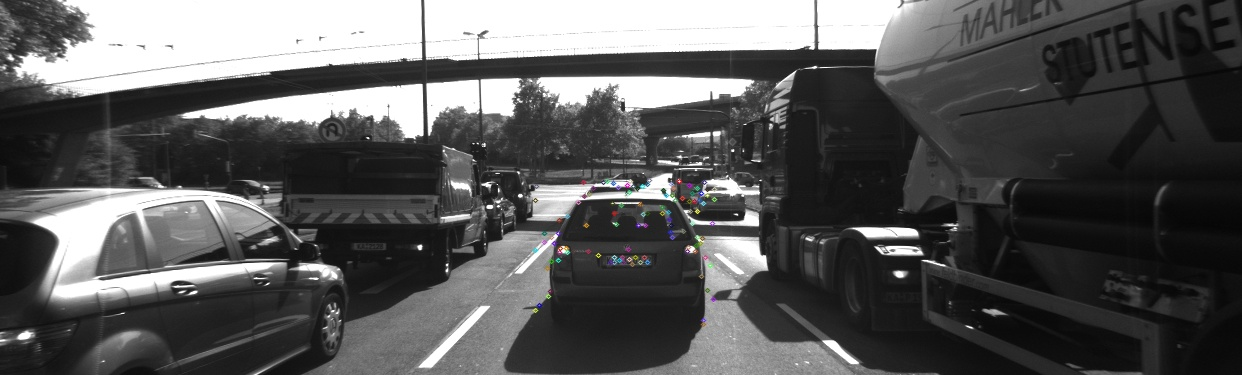
\includegraphics[width=0.8\columnwidth]{./keypoints/SHITOMASI}
	\caption{Shi-Tomasi keypoints.}
	\label{fig:shi_tomasi_keypoints}
\end{figure}

\begin{figure}
	\centering
	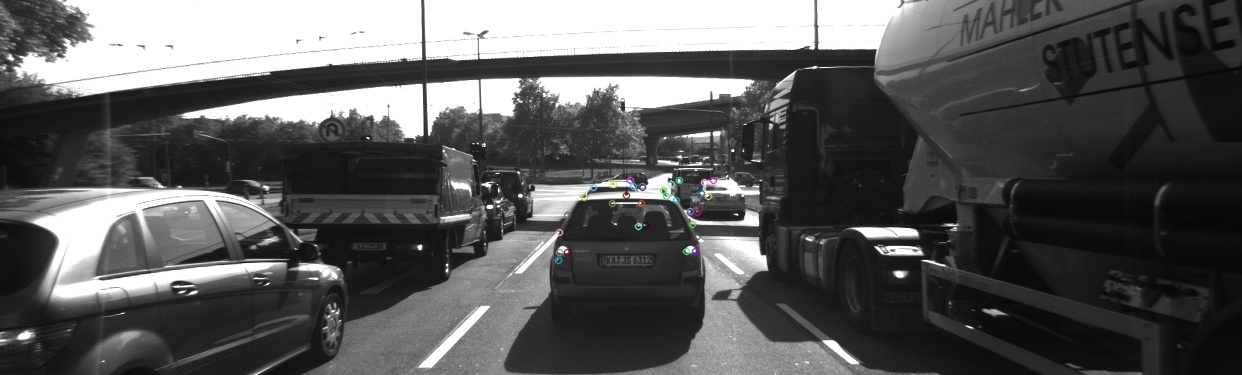
\includegraphics[width=0.8\columnwidth]{./keypoints/HARRIS}
	\caption{Harris keypoints.}
\end{figure}

\begin{figure}
	\centering
	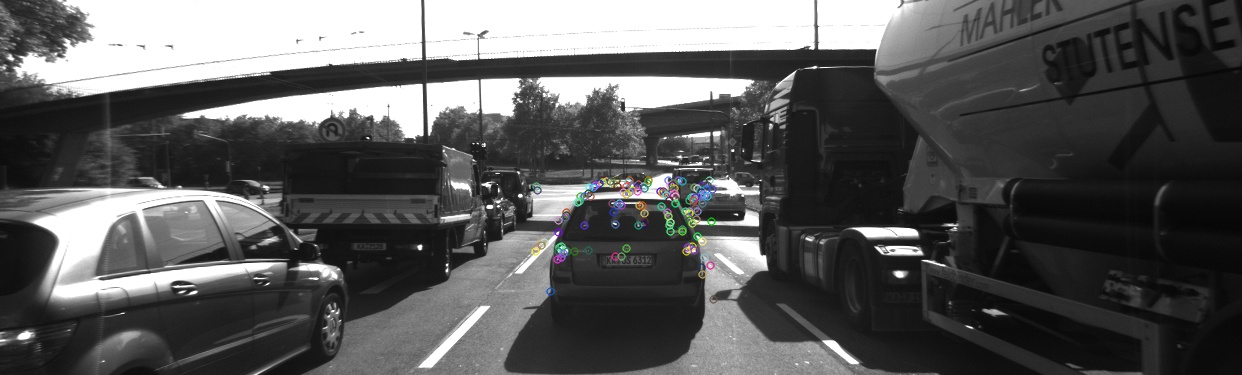
\includegraphics[width=0.8\columnwidth]{./keypoints/FAST}
	\caption{FAST keypoints.}
\end{figure}

\begin{figure}
	\centering
	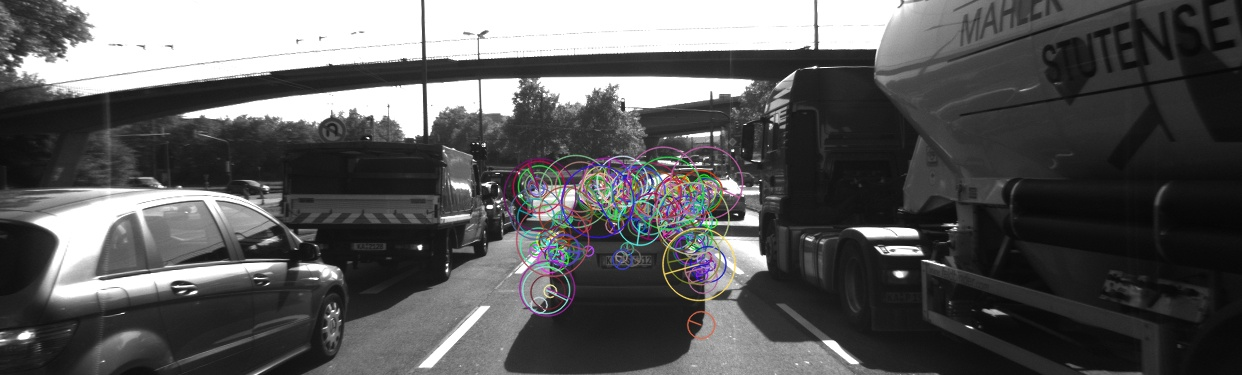
\includegraphics[width=0.8\columnwidth]{./keypoints/BRISK}
	\caption{BRISK keypoints.}
\end{figure}

\begin{figure}
	\centering
	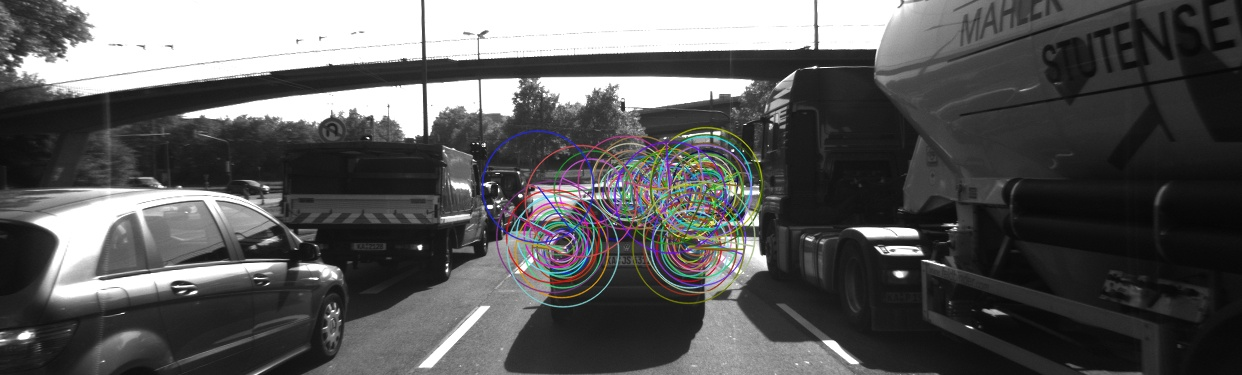
\includegraphics[width=0.8\columnwidth]{./keypoints/ORB}
	\caption{ORB keypoints.}
\end{figure}

\begin{figure}
	\centering
	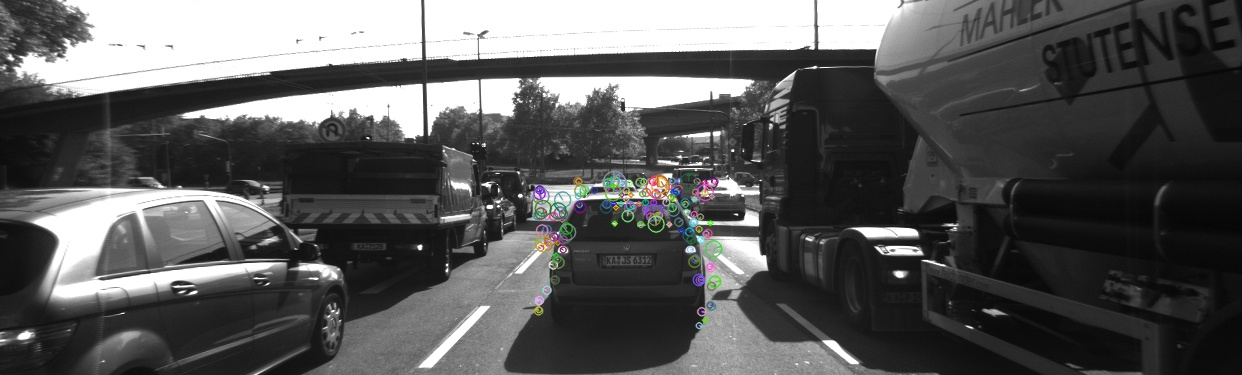
\includegraphics[width=0.8\columnwidth]{./keypoints/AKAZE}
	\caption{AKAZE keypoints.}
\end{figure}

\begin{figure}
	\centering
	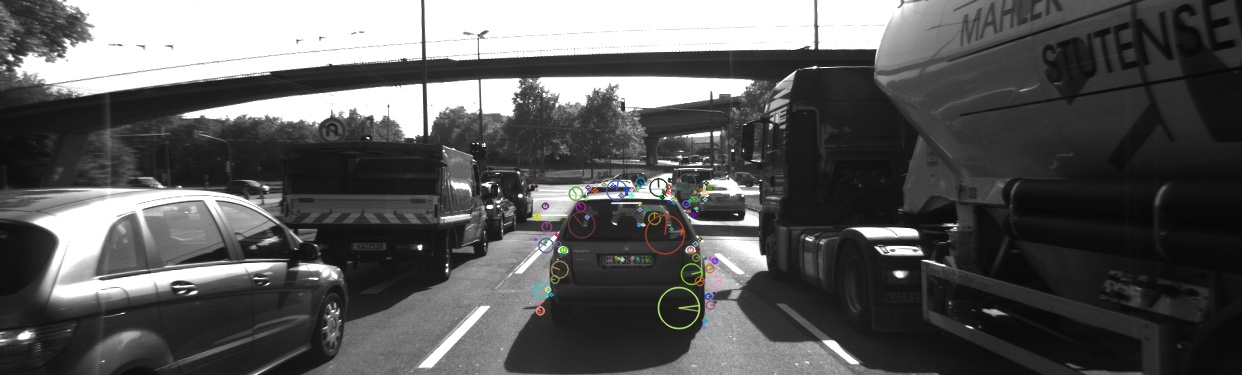
\includegraphics[width=0.8\columnwidth]{./keypoints/SIFT}
	\caption{SIFT keypoints.}
	\label{fig:sift_keypoints}
\end{figure}

\subsection*{MP.8 Performance Evaluation 2}
\textcolor{gray}{\textit{Count the number of matched keypoints for all 10 images using all possible combinations of detectors and descriptors. In the matching step, the BF approach is used with the descriptor distance ratio set to 0.8.}}


\subsection*{MP.9 Performance Evaluation 3}
\textcolor{gray}{\textit{Log the time it takes for keypoint detection and descriptor extraction. The results must be entered into a spreadsheet and based on this data, the TOP3 detector / descriptor combinations must be recommended as the best choice for our purpose of detecting keypoints on vehicles.}}


\end{document}